\title{Ex Vb - sheet 5}
\author{Luca Cordes, 444900}
\documentclass[11pt]{article}

    \usepackage[breakable]{tcolorbox}
    \usepackage{parskip} % Stop auto-indenting (to mimic markdown behaviour)
    

    % Basic figure setup, for now with no caption control since it's done
    % automatically by Pandoc (which extracts ![](path) syntax from Markdown).
    \usepackage{graphicx}
    % Keep aspect ratio if custom image width or height is specified
    \setkeys{Gin}{keepaspectratio}
    % Maintain compatibility with old templates. Remove in nbconvert 6.0
    \let\Oldincludegraphics\includegraphics
    % Ensure that by default, figures have no caption (until we provide a
    % proper Figure object with a Caption API and a way to capture that
    % in the conversion process - todo).
    \usepackage{caption}
    \DeclareCaptionFormat{nocaption}{}
    \captionsetup{format=nocaption,aboveskip=0pt,belowskip=0pt}

    \usepackage{float}
    \floatplacement{figure}{H} % forces figures to be placed at the correct location
    \usepackage{xcolor} % Allow colors to be defined
    \usepackage{enumerate} % Needed for markdown enumerations to work
    \usepackage{geometry} % Used to adjust the document margins
    \usepackage{amsmath} % Equations
    \usepackage{amssymb} % Equations
    \usepackage{textcomp} % defines textquotesingle
    % Hack from http://tex.stackexchange.com/a/47451/13684:
    \AtBeginDocument{%
        \def\PYZsq{\textquotesingle}% Upright quotes in Pygmentized code
    }
    \usepackage{upquote} % Upright quotes for verbatim code
    \usepackage{eurosym} % defines \euro

    \usepackage{iftex}
    \ifPDFTeX
        \usepackage[T1]{fontenc}
        \IfFileExists{alphabeta.sty}{
              \usepackage{alphabeta}
          }{
              \usepackage[mathletters]{ucs}
              \usepackage[utf8x]{inputenc}
          }
    \else
        \usepackage{fontspec}
        \usepackage{unicode-math}
    \fi

    \usepackage{fancyvrb} % verbatim replacement that allows latex
    \usepackage{grffile} % extends the file name processing of package graphics
                         % to support a larger range
    \makeatletter % fix for old versions of grffile with XeLaTeX
    \@ifpackagelater{grffile}{2019/11/01}
    {
      % Do nothing on new versions
    }
    {
      \def\Gread@@xetex#1{%
        \IfFileExists{"\Gin@base".bb}%
        {\Gread@eps{\Gin@base.bb}}%
        {\Gread@@xetex@aux#1}%
      }
    }
    \makeatother
    \usepackage[Export]{adjustbox} % Used to constrain images to a maximum size
    \adjustboxset{max size={0.9\linewidth}{0.9\paperheight}}

    % The hyperref package gives us a pdf with properly built
    % internal navigation ('pdf bookmarks' for the table of contents,
    % internal cross-reference links, web links for URLs, etc.)
    \usepackage{hyperref}
    % The default LaTeX title has an obnoxious amount of whitespace. By default,
    % titling removes some of it. It also provides customization options.
    \usepackage{titling}
    \usepackage{longtable} % longtable support required by pandoc >1.10
    \usepackage{booktabs}  % table support for pandoc > 1.12.2
    \usepackage{array}     % table support for pandoc >= 2.11.3
    \usepackage{calc}      % table minipage width calculation for pandoc >= 2.11.1
    \usepackage[inline]{enumitem} % IRkernel/repr support (it uses the enumerate* environment)
    \usepackage[normalem]{ulem} % ulem is needed to support strikethroughs (\sout)
                                % normalem makes italics be italics, not underlines
    \usepackage{soul}      % strikethrough (\st) support for pandoc >= 3.0.0
    \usepackage{mathrsfs}
    

    
    % Colors for the hyperref package
    \definecolor{urlcolor}{rgb}{0,.145,.698}
    \definecolor{linkcolor}{rgb}{.71,0.21,0.01}
    \definecolor{citecolor}{rgb}{.12,.54,.11}

    % ANSI colors
    \definecolor{ansi-black}{HTML}{3E424D}
    \definecolor{ansi-black-intense}{HTML}{282C36}
    \definecolor{ansi-red}{HTML}{E75C58}
    \definecolor{ansi-red-intense}{HTML}{B22B31}
    \definecolor{ansi-green}{HTML}{00A250}
    \definecolor{ansi-green-intense}{HTML}{007427}
    \definecolor{ansi-yellow}{HTML}{DDB62B}
    \definecolor{ansi-yellow-intense}{HTML}{B27D12}
    \definecolor{ansi-blue}{HTML}{208FFB}
    \definecolor{ansi-blue-intense}{HTML}{0065CA}
    \definecolor{ansi-magenta}{HTML}{D160C4}
    \definecolor{ansi-magenta-intense}{HTML}{A03196}
    \definecolor{ansi-cyan}{HTML}{60C6C8}
    \definecolor{ansi-cyan-intense}{HTML}{258F8F}
    \definecolor{ansi-white}{HTML}{C5C1B4}
    \definecolor{ansi-white-intense}{HTML}{A1A6B2}
    \definecolor{ansi-default-inverse-fg}{HTML}{FFFFFF}
    \definecolor{ansi-default-inverse-bg}{HTML}{000000}

    % common color for the border for error outputs.
    \definecolor{outerrorbackground}{HTML}{FFDFDF}

    % commands and environments needed by pandoc snippets
    % extracted from the output of `pandoc -s`
    \providecommand{\tightlist}{%
      \setlength{\itemsep}{0pt}\setlength{\parskip}{0pt}}
    \DefineVerbatimEnvironment{Highlighting}{Verbatim}{commandchars=\\\{\}}
    % Add ',fontsize=\small' for more characters per line
    \newenvironment{Shaded}{}{}
    \newcommand{\KeywordTok}[1]{\textcolor[rgb]{0.00,0.44,0.13}{\textbf{{#1}}}}
    \newcommand{\DataTypeTok}[1]{\textcolor[rgb]{0.56,0.13,0.00}{{#1}}}
    \newcommand{\DecValTok}[1]{\textcolor[rgb]{0.25,0.63,0.44}{{#1}}}
    \newcommand{\BaseNTok}[1]{\textcolor[rgb]{0.25,0.63,0.44}{{#1}}}
    \newcommand{\FloatTok}[1]{\textcolor[rgb]{0.25,0.63,0.44}{{#1}}}
    \newcommand{\CharTok}[1]{\textcolor[rgb]{0.25,0.44,0.63}{{#1}}}
    \newcommand{\StringTok}[1]{\textcolor[rgb]{0.25,0.44,0.63}{{#1}}}
    \newcommand{\CommentTok}[1]{\textcolor[rgb]{0.38,0.63,0.69}{\textit{{#1}}}}
    \newcommand{\OtherTok}[1]{\textcolor[rgb]{0.00,0.44,0.13}{{#1}}}
    \newcommand{\AlertTok}[1]{\textcolor[rgb]{1.00,0.00,0.00}{\textbf{{#1}}}}
    \newcommand{\FunctionTok}[1]{\textcolor[rgb]{0.02,0.16,0.49}{{#1}}}
    \newcommand{\RegionMarkerTok}[1]{{#1}}
    \newcommand{\ErrorTok}[1]{\textcolor[rgb]{1.00,0.00,0.00}{\textbf{{#1}}}}
    \newcommand{\NormalTok}[1]{{#1}}

    % Additional commands for more recent versions of Pandoc
    \newcommand{\ConstantTok}[1]{\textcolor[rgb]{0.53,0.00,0.00}{{#1}}}
    \newcommand{\SpecialCharTok}[1]{\textcolor[rgb]{0.25,0.44,0.63}{{#1}}}
    \newcommand{\VerbatimStringTok}[1]{\textcolor[rgb]{0.25,0.44,0.63}{{#1}}}
    \newcommand{\SpecialStringTok}[1]{\textcolor[rgb]{0.73,0.40,0.53}{{#1}}}
    \newcommand{\ImportTok}[1]{{#1}}
    \newcommand{\DocumentationTok}[1]{\textcolor[rgb]{0.73,0.13,0.13}{\textit{{#1}}}}
    \newcommand{\AnnotationTok}[1]{\textcolor[rgb]{0.38,0.63,0.69}{\textbf{\textit{{#1}}}}}
    \newcommand{\CommentVarTok}[1]{\textcolor[rgb]{0.38,0.63,0.69}{\textbf{\textit{{#1}}}}}
    \newcommand{\VariableTok}[1]{\textcolor[rgb]{0.10,0.09,0.49}{{#1}}}
    \newcommand{\ControlFlowTok}[1]{\textcolor[rgb]{0.00,0.44,0.13}{\textbf{{#1}}}}
    \newcommand{\OperatorTok}[1]{\textcolor[rgb]{0.40,0.40,0.40}{{#1}}}
    \newcommand{\BuiltInTok}[1]{{#1}}
    \newcommand{\ExtensionTok}[1]{{#1}}
    \newcommand{\PreprocessorTok}[1]{\textcolor[rgb]{0.74,0.48,0.00}{{#1}}}
    \newcommand{\AttributeTok}[1]{\textcolor[rgb]{0.49,0.56,0.16}{{#1}}}
    \newcommand{\InformationTok}[1]{\textcolor[rgb]{0.38,0.63,0.69}{\textbf{\textit{{#1}}}}}
    \newcommand{\WarningTok}[1]{\textcolor[rgb]{0.38,0.63,0.69}{\textbf{\textit{{#1}}}}}


    % Define a nice break command that doesn't care if a line doesn't already
    % exist.
    \def\br{\hspace*{\fill} \\* }
    % Math Jax compatibility definitions
    \def\gt{>}
    \def\lt{<}
    \let\Oldtex\TeX
    \let\Oldlatex\LaTeX
    \renewcommand{\TeX}{\textrm{\Oldtex}}
    \renewcommand{\LaTeX}{\textrm{\Oldlatex}}
    % Document parameters
    % Document title
    
    
    
% Pygments definitions
\makeatletter
\def\PY@reset{\let\PY@it=\relax \let\PY@bf=\relax%
    \let\PY@ul=\relax \let\PY@tc=\relax%
    \let\PY@bc=\relax \let\PY@ff=\relax}
\def\PY@tok#1{\csname PY@tok@#1\endcsname}
\def\PY@toks#1+{\ifx\relax#1\empty\else%
    \PY@tok{#1}\expandafter\PY@toks\fi}
\def\PY@do#1{\PY@bc{\PY@tc{\PY@ul{%
    \PY@it{\PY@bf{\PY@ff{#1}}}}}}}
\def\PY#1#2{\PY@reset\PY@toks#1+\relax+\PY@do{#2}}

\@namedef{PY@tok@w}{\def\PY@tc##1{\textcolor[rgb]{0.73,0.73,0.73}{##1}}}
\@namedef{PY@tok@c}{\let\PY@it=\textit\def\PY@tc##1{\textcolor[rgb]{0.24,0.48,0.48}{##1}}}
\@namedef{PY@tok@cp}{\def\PY@tc##1{\textcolor[rgb]{0.61,0.40,0.00}{##1}}}
\@namedef{PY@tok@k}{\let\PY@bf=\textbf\def\PY@tc##1{\textcolor[rgb]{0.00,0.50,0.00}{##1}}}
\@namedef{PY@tok@kp}{\def\PY@tc##1{\textcolor[rgb]{0.00,0.50,0.00}{##1}}}
\@namedef{PY@tok@kt}{\def\PY@tc##1{\textcolor[rgb]{0.69,0.00,0.25}{##1}}}
\@namedef{PY@tok@o}{\def\PY@tc##1{\textcolor[rgb]{0.40,0.40,0.40}{##1}}}
\@namedef{PY@tok@ow}{\let\PY@bf=\textbf\def\PY@tc##1{\textcolor[rgb]{0.67,0.13,1.00}{##1}}}
\@namedef{PY@tok@nb}{\def\PY@tc##1{\textcolor[rgb]{0.00,0.50,0.00}{##1}}}
\@namedef{PY@tok@nf}{\def\PY@tc##1{\textcolor[rgb]{0.00,0.00,1.00}{##1}}}
\@namedef{PY@tok@nc}{\let\PY@bf=\textbf\def\PY@tc##1{\textcolor[rgb]{0.00,0.00,1.00}{##1}}}
\@namedef{PY@tok@nn}{\let\PY@bf=\textbf\def\PY@tc##1{\textcolor[rgb]{0.00,0.00,1.00}{##1}}}
\@namedef{PY@tok@ne}{\let\PY@bf=\textbf\def\PY@tc##1{\textcolor[rgb]{0.80,0.25,0.22}{##1}}}
\@namedef{PY@tok@nv}{\def\PY@tc##1{\textcolor[rgb]{0.10,0.09,0.49}{##1}}}
\@namedef{PY@tok@no}{\def\PY@tc##1{\textcolor[rgb]{0.53,0.00,0.00}{##1}}}
\@namedef{PY@tok@nl}{\def\PY@tc##1{\textcolor[rgb]{0.46,0.46,0.00}{##1}}}
\@namedef{PY@tok@ni}{\let\PY@bf=\textbf\def\PY@tc##1{\textcolor[rgb]{0.44,0.44,0.44}{##1}}}
\@namedef{PY@tok@na}{\def\PY@tc##1{\textcolor[rgb]{0.41,0.47,0.13}{##1}}}
\@namedef{PY@tok@nt}{\let\PY@bf=\textbf\def\PY@tc##1{\textcolor[rgb]{0.00,0.50,0.00}{##1}}}
\@namedef{PY@tok@nd}{\def\PY@tc##1{\textcolor[rgb]{0.67,0.13,1.00}{##1}}}
\@namedef{PY@tok@s}{\def\PY@tc##1{\textcolor[rgb]{0.73,0.13,0.13}{##1}}}
\@namedef{PY@tok@sd}{\let\PY@it=\textit\def\PY@tc##1{\textcolor[rgb]{0.73,0.13,0.13}{##1}}}
\@namedef{PY@tok@si}{\let\PY@bf=\textbf\def\PY@tc##1{\textcolor[rgb]{0.64,0.35,0.47}{##1}}}
\@namedef{PY@tok@se}{\let\PY@bf=\textbf\def\PY@tc##1{\textcolor[rgb]{0.67,0.36,0.12}{##1}}}
\@namedef{PY@tok@sr}{\def\PY@tc##1{\textcolor[rgb]{0.64,0.35,0.47}{##1}}}
\@namedef{PY@tok@ss}{\def\PY@tc##1{\textcolor[rgb]{0.10,0.09,0.49}{##1}}}
\@namedef{PY@tok@sx}{\def\PY@tc##1{\textcolor[rgb]{0.00,0.50,0.00}{##1}}}
\@namedef{PY@tok@m}{\def\PY@tc##1{\textcolor[rgb]{0.40,0.40,0.40}{##1}}}
\@namedef{PY@tok@gh}{\let\PY@bf=\textbf\def\PY@tc##1{\textcolor[rgb]{0.00,0.00,0.50}{##1}}}
\@namedef{PY@tok@gu}{\let\PY@bf=\textbf\def\PY@tc##1{\textcolor[rgb]{0.50,0.00,0.50}{##1}}}
\@namedef{PY@tok@gd}{\def\PY@tc##1{\textcolor[rgb]{0.63,0.00,0.00}{##1}}}
\@namedef{PY@tok@gi}{\def\PY@tc##1{\textcolor[rgb]{0.00,0.52,0.00}{##1}}}
\@namedef{PY@tok@gr}{\def\PY@tc##1{\textcolor[rgb]{0.89,0.00,0.00}{##1}}}
\@namedef{PY@tok@ge}{\let\PY@it=\textit}
\@namedef{PY@tok@gs}{\let\PY@bf=\textbf}
\@namedef{PY@tok@ges}{\let\PY@bf=\textbf\let\PY@it=\textit}
\@namedef{PY@tok@gp}{\let\PY@bf=\textbf\def\PY@tc##1{\textcolor[rgb]{0.00,0.00,0.50}{##1}}}
\@namedef{PY@tok@go}{\def\PY@tc##1{\textcolor[rgb]{0.44,0.44,0.44}{##1}}}
\@namedef{PY@tok@gt}{\def\PY@tc##1{\textcolor[rgb]{0.00,0.27,0.87}{##1}}}
\@namedef{PY@tok@err}{\def\PY@bc##1{{\setlength{\fboxsep}{\string -\fboxrule}\fcolorbox[rgb]{1.00,0.00,0.00}{1,1,1}{\strut ##1}}}}
\@namedef{PY@tok@kc}{\let\PY@bf=\textbf\def\PY@tc##1{\textcolor[rgb]{0.00,0.50,0.00}{##1}}}
\@namedef{PY@tok@kd}{\let\PY@bf=\textbf\def\PY@tc##1{\textcolor[rgb]{0.00,0.50,0.00}{##1}}}
\@namedef{PY@tok@kn}{\let\PY@bf=\textbf\def\PY@tc##1{\textcolor[rgb]{0.00,0.50,0.00}{##1}}}
\@namedef{PY@tok@kr}{\let\PY@bf=\textbf\def\PY@tc##1{\textcolor[rgb]{0.00,0.50,0.00}{##1}}}
\@namedef{PY@tok@bp}{\def\PY@tc##1{\textcolor[rgb]{0.00,0.50,0.00}{##1}}}
\@namedef{PY@tok@fm}{\def\PY@tc##1{\textcolor[rgb]{0.00,0.00,1.00}{##1}}}
\@namedef{PY@tok@vc}{\def\PY@tc##1{\textcolor[rgb]{0.10,0.09,0.49}{##1}}}
\@namedef{PY@tok@vg}{\def\PY@tc##1{\textcolor[rgb]{0.10,0.09,0.49}{##1}}}
\@namedef{PY@tok@vi}{\def\PY@tc##1{\textcolor[rgb]{0.10,0.09,0.49}{##1}}}
\@namedef{PY@tok@vm}{\def\PY@tc##1{\textcolor[rgb]{0.10,0.09,0.49}{##1}}}
\@namedef{PY@tok@sa}{\def\PY@tc##1{\textcolor[rgb]{0.73,0.13,0.13}{##1}}}
\@namedef{PY@tok@sb}{\def\PY@tc##1{\textcolor[rgb]{0.73,0.13,0.13}{##1}}}
\@namedef{PY@tok@sc}{\def\PY@tc##1{\textcolor[rgb]{0.73,0.13,0.13}{##1}}}
\@namedef{PY@tok@dl}{\def\PY@tc##1{\textcolor[rgb]{0.73,0.13,0.13}{##1}}}
\@namedef{PY@tok@s2}{\def\PY@tc##1{\textcolor[rgb]{0.73,0.13,0.13}{##1}}}
\@namedef{PY@tok@sh}{\def\PY@tc##1{\textcolor[rgb]{0.73,0.13,0.13}{##1}}}
\@namedef{PY@tok@s1}{\def\PY@tc##1{\textcolor[rgb]{0.73,0.13,0.13}{##1}}}
\@namedef{PY@tok@mb}{\def\PY@tc##1{\textcolor[rgb]{0.40,0.40,0.40}{##1}}}
\@namedef{PY@tok@mf}{\def\PY@tc##1{\textcolor[rgb]{0.40,0.40,0.40}{##1}}}
\@namedef{PY@tok@mh}{\def\PY@tc##1{\textcolor[rgb]{0.40,0.40,0.40}{##1}}}
\@namedef{PY@tok@mi}{\def\PY@tc##1{\textcolor[rgb]{0.40,0.40,0.40}{##1}}}
\@namedef{PY@tok@il}{\def\PY@tc##1{\textcolor[rgb]{0.40,0.40,0.40}{##1}}}
\@namedef{PY@tok@mo}{\def\PY@tc##1{\textcolor[rgb]{0.40,0.40,0.40}{##1}}}
\@namedef{PY@tok@ch}{\let\PY@it=\textit\def\PY@tc##1{\textcolor[rgb]{0.24,0.48,0.48}{##1}}}
\@namedef{PY@tok@cm}{\let\PY@it=\textit\def\PY@tc##1{\textcolor[rgb]{0.24,0.48,0.48}{##1}}}
\@namedef{PY@tok@cpf}{\let\PY@it=\textit\def\PY@tc##1{\textcolor[rgb]{0.24,0.48,0.48}{##1}}}
\@namedef{PY@tok@c1}{\let\PY@it=\textit\def\PY@tc##1{\textcolor[rgb]{0.24,0.48,0.48}{##1}}}
\@namedef{PY@tok@cs}{\let\PY@it=\textit\def\PY@tc##1{\textcolor[rgb]{0.24,0.48,0.48}{##1}}}

\def\PYZbs{\char`\\}
\def\PYZus{\char`\_}
\def\PYZob{\char`\{}
\def\PYZcb{\char`\}}
\def\PYZca{\char`\^}
\def\PYZam{\char`\&}
\def\PYZlt{\char`\<}
\def\PYZgt{\char`\>}
\def\PYZsh{\char`\#}
\def\PYZpc{\char`\%}
\def\PYZdl{\char`\$}
\def\PYZhy{\char`\-}
\def\PYZsq{\char`\'}
\def\PYZdq{\char`\"}
\def\PYZti{\char`\~}
% for compatibility with earlier versions
\def\PYZat{@}
\def\PYZlb{[}
\def\PYZrb{]}
\makeatother


    % For linebreaks inside Verbatim environment from package fancyvrb.
    \makeatletter
        \newbox\Wrappedcontinuationbox
        \newbox\Wrappedvisiblespacebox
        \newcommand*\Wrappedvisiblespace {\textcolor{red}{\textvisiblespace}}
        \newcommand*\Wrappedcontinuationsymbol {\textcolor{red}{\llap{\tiny$\m@th\hookrightarrow$}}}
        \newcommand*\Wrappedcontinuationindent {3ex }
        \newcommand*\Wrappedafterbreak {\kern\Wrappedcontinuationindent\copy\Wrappedcontinuationbox}
        % Take advantage of the already applied Pygments mark-up to insert
        % potential linebreaks for TeX processing.
        %        {, <, #, %, $, ' and ": go to next line.
        %        _, }, ^, &, >, - and ~: stay at end of broken line.
        % Use of \textquotesingle for straight quote.
        \newcommand*\Wrappedbreaksatspecials {%
            \def\PYGZus{\discretionary{\char`\_}{\Wrappedafterbreak}{\char`\_}}%
            \def\PYGZob{\discretionary{}{\Wrappedafterbreak\char`\{}{\char`\{}}%
            \def\PYGZcb{\discretionary{\char`\}}{\Wrappedafterbreak}{\char`\}}}%
            \def\PYGZca{\discretionary{\char`\^}{\Wrappedafterbreak}{\char`\^}}%
            \def\PYGZam{\discretionary{\char`\&}{\Wrappedafterbreak}{\char`\&}}%
            \def\PYGZlt{\discretionary{}{\Wrappedafterbreak\char`\<}{\char`\<}}%
            \def\PYGZgt{\discretionary{\char`\>}{\Wrappedafterbreak}{\char`\>}}%
            \def\PYGZsh{\discretionary{}{\Wrappedafterbreak\char`\#}{\char`\#}}%
            \def\PYGZpc{\discretionary{}{\Wrappedafterbreak\char`\%}{\char`\%}}%
            \def\PYGZdl{\discretionary{}{\Wrappedafterbreak\char`\$}{\char`\$}}%
            \def\PYGZhy{\discretionary{\char`\-}{\Wrappedafterbreak}{\char`\-}}%
            \def\PYGZsq{\discretionary{}{\Wrappedafterbreak\textquotesingle}{\textquotesingle}}%
            \def\PYGZdq{\discretionary{}{\Wrappedafterbreak\char`\"}{\char`\"}}%
            \def\PYGZti{\discretionary{\char`\~}{\Wrappedafterbreak}{\char`\~}}%
        }
        % Some characters . , ; ? ! / are not pygmentized.
        % This macro makes them "active" and they will insert potential linebreaks
        \newcommand*\Wrappedbreaksatpunct {%
            \lccode`\~`\.\lowercase{\def~}{\discretionary{\hbox{\char`\.}}{\Wrappedafterbreak}{\hbox{\char`\.}}}%
            \lccode`\~`\,\lowercase{\def~}{\discretionary{\hbox{\char`\,}}{\Wrappedafterbreak}{\hbox{\char`\,}}}%
            \lccode`\~`\;\lowercase{\def~}{\discretionary{\hbox{\char`\;}}{\Wrappedafterbreak}{\hbox{\char`\;}}}%
            \lccode`\~`\:\lowercase{\def~}{\discretionary{\hbox{\char`\:}}{\Wrappedafterbreak}{\hbox{\char`\:}}}%
            \lccode`\~`\?\lowercase{\def~}{\discretionary{\hbox{\char`\?}}{\Wrappedafterbreak}{\hbox{\char`\?}}}%
            \lccode`\~`\!\lowercase{\def~}{\discretionary{\hbox{\char`\!}}{\Wrappedafterbreak}{\hbox{\char`\!}}}%
            \lccode`\~`\/\lowercase{\def~}{\discretionary{\hbox{\char`\/}}{\Wrappedafterbreak}{\hbox{\char`\/}}}%
            \catcode`\.\active
            \catcode`\,\active
            \catcode`\;\active
            \catcode`\:\active
            \catcode`\?\active
            \catcode`\!\active
            \catcode`\/\active
            \lccode`\~`\~
        }
    \makeatother

    \let\OriginalVerbatim=\Verbatim
    \makeatletter
    \renewcommand{\Verbatim}[1][1]{%
        %\parskip\z@skip
        \sbox\Wrappedcontinuationbox {\Wrappedcontinuationsymbol}%
        \sbox\Wrappedvisiblespacebox {\FV@SetupFont\Wrappedvisiblespace}%
        \def\FancyVerbFormatLine ##1{\hsize\linewidth
            \vtop{\raggedright\hyphenpenalty\z@\exhyphenpenalty\z@
                \doublehyphendemerits\z@\finalhyphendemerits\z@
                \strut ##1\strut}%
        }%
        % If the linebreak is at a space, the latter will be displayed as visible
        % space at end of first line, and a continuation symbol starts next line.
        % Stretch/shrink are however usually zero for typewriter font.
        \def\FV@Space {%
            \nobreak\hskip\z@ plus\fontdimen3\font minus\fontdimen4\font
            \discretionary{\copy\Wrappedvisiblespacebox}{\Wrappedafterbreak}
            {\kern\fontdimen2\font}%
        }%

        % Allow breaks at special characters using \PYG... macros.
        \Wrappedbreaksatspecials
        % Breaks at punctuation characters . , ; ? ! and / need catcode=\active
        \OriginalVerbatim[#1,codes*=\Wrappedbreaksatpunct]%
    }
    \makeatother

    % Exact colors from NB
    \definecolor{incolor}{HTML}{303F9F}
    \definecolor{outcolor}{HTML}{D84315}
    \definecolor{cellborder}{HTML}{CFCFCF}
    \definecolor{cellbackground}{HTML}{F7F7F7}

    % prompt
    \makeatletter
    \newcommand{\boxspacing}{\kern\kvtcb@left@rule\kern\kvtcb@boxsep}
    \makeatother
    \newcommand{\prompt}[4]{
        {\ttfamily\llap{{\color{#2}[#3]:\hspace{3pt}#4}}\vspace{-\baselineskip}}
    }
    

    
    % Prevent overflowing lines due to hard-to-break entities
    \sloppy
    % Setup hyperref package
    \hypersetup{
      breaklinks=true,  % so long urls are correctly broken across lines
      colorlinks=true,
      urlcolor=urlcolor,
      linkcolor=linkcolor,
      citecolor=citecolor,
      }
    % Slightly bigger margins than the latex defaults
    
    \geometry{verbose,tmargin=1in,bmargin=1in,lmargin=1in,rmargin=1in}
    
    

\begin{document}
    
    \maketitle
    
    \begin{tcolorbox}[breakable, size=fbox, boxrule=1pt, pad at break*=1mm,colback=cellbackground, colframe=cellborder]
\prompt{In}{incolor}{1}{\boxspacing}
\begin{Verbatim}[commandchars=\\\{\}]
\PY{k+kn}{from} \PY{n+nn}{sympy} \PY{k+kn}{import} \PY{o}{*}
\PY{k+kn}{import} \PY{n+nn}{numpy} \PY{k}{as} \PY{n+nn}{np} 
\PY{k+kn}{import} \PY{n+nn}{scipy}\PY{n+nn}{.}\PY{n+nn}{constants} \PY{k}{as} \PY{n+nn}{c}
\PY{k+kn}{from} \PY{n+nn}{IPython}\PY{n+nn}{.}\PY{n+nn}{display} \PY{k+kn}{import} \PY{n}{display} \PY{k}{as} \PY{n+nb}{print}
\PY{n}{init\PYZus{}printing}\PY{p}{(}\PY{n}{use\PYZus{}latex}\PY{o}{=}\PY{l+s+s2}{\PYZdq{}}\PY{l+s+s2}{mathjax}\PY{l+s+s2}{\PYZdq{}}\PY{p}{)}
\end{Verbatim}
\end{tcolorbox}

    \hypertarget{nr.-1-electron-muon-scattering}{%
\section{Nr. 1
Electron-muon-scattering}\label{nr.-1-electron-muon-scattering}}

    The number of particles per second is \(W = L \sigma\), where \(\sigma\)
is the differential cross section integrated over the central region
\(\sigma = \int_{45^\circ}^{135^\circ} \mathrm d\theta\,2\pi\sin(\theta) \frac{\mathrm d \sigma}{\mathrm d \Omega}\).

    \begin{tcolorbox}[breakable, size=fbox, boxrule=1pt, pad at break*=1mm,colback=cellbackground, colframe=cellborder]
\prompt{In}{incolor}{2}{\boxspacing}
\begin{Verbatim}[commandchars=\\\{\}]
\PY{n}{s}\PY{p}{,}\PY{n}{L}\PY{p}{,}\PY{n}{theta}\PY{p}{,}\PY{n}{alpha} \PY{o}{=} \PY{n}{symbols}\PY{p}{(}\PY{l+s+s2}{\PYZdq{}}\PY{l+s+s2}{s L theta alpha}\PY{l+s+s2}{\PYZdq{}}\PY{p}{)}
\PY{n}{deg} \PY{o}{=} \PY{l+m+mi}{2}\PY{o}{*}\PY{n}{pi}\PY{o}{/}\PY{l+m+mi}{360}
\PY{n}{gev\PYZus{}to\PYZus{}cm2} \PY{o}{=} \PY{p}{(}\PY{n}{c}\PY{o}{.}\PY{n}{c} \PY{o}{*} \PY{n}{c}\PY{o}{.}\PY{n}{hbar} \PY{o}{/} \PY{p}{(}\PY{n}{c}\PY{o}{.}\PY{n}{e} \PY{o}{*} \PY{l+m+mf}{1e9}\PY{p}{)}\PY{p}{)}\PY{o}{*}\PY{o}{*}\PY{l+m+mi}{2} \PY{o}{*} \PY{p}{(}\PY{l+m+mf}{1e2}\PY{p}{)}\PY{o}{*}\PY{o}{*}\PY{l+m+mi}{2} \PY{c+c1}{\PYZsh{} GeV\PYZca{}\PYZhy{}2 to cm\PYZca{}2}

\PY{n}{subs} \PY{o}{=} \PY{p}{\PYZob{}}\PY{n}{s}\PY{p}{:} \PY{l+m+mi}{34}\PY{o}{*}\PY{o}{*}\PY{l+m+mi}{2}\PY{p}{,} \PY{c+c1}{\PYZsh{} GeV\PYZca{}2}
        \PY{n}{L}\PY{p}{:} \PY{l+m+mf}{5e30}\PY{p}{,} \PY{c+c1}{\PYZsh{} cm\PYZca{}\PYZhy{}2 s\PYZca{}\PYZhy{}1}
        \PY{n}{alpha}\PY{p}{:} \PY{n}{c}\PY{o}{.}\PY{n}{alpha}\PY{p}{\PYZcb{}}
\PY{n}{diff\PYZus{}cross\PYZus{}section} \PY{o}{=} \PY{n}{alpha}\PY{o}{*}\PY{o}{*}\PY{l+m+mi}{2}\PY{o}{/}\PY{p}{(}\PY{l+m+mi}{4}\PY{o}{*}\PY{n}{s}\PY{p}{)} \PY{o}{*} \PY{p}{(}\PY{l+m+mi}{1} \PY{o}{+} \PY{n}{cos}\PY{p}{(}\PY{n}{theta}\PY{p}{)}\PY{o}{*}\PY{o}{*}\PY{l+m+mi}{2}\PY{p}{)}

\PY{n}{cross\PYZus{}section} \PY{o}{=} \PY{n}{Integral}\PY{p}{(}\PY{p}{(}\PY{l+m+mi}{2}\PY{o}{*}\PY{n}{pi}\PY{o}{*}\PY{n}{sin}\PY{p}{(}\PY{n}{theta}\PY{p}{)}\PY{o}{*}\PY{n}{diff\PYZus{}cross\PYZus{}section}\PY{p}{)}\PY{p}{,}\PY{p}{(}\PY{n}{theta}\PY{p}{,} \PY{l+m+mi}{45}\PY{o}{*}\PY{n}{deg}\PY{p}{,} \PY{l+m+mi}{135}\PY{o}{*}\PY{n}{deg}\PY{p}{)}\PY{p}{)}
\PY{n}{cross\PYZus{}section}
\end{Verbatim}
\end{tcolorbox}
 
            
\prompt{Out}{outcolor}{2}{}
    
    $\displaystyle \int\limits_{\frac{\pi}{4}}^{\frac{3 \pi}{4}} \frac{\pi \alpha^{2} \left(\cos^{2}{\left(\theta \right)} + 1\right) \sin{\left(\theta \right)}}{2 s}\, d\theta$

    

    \begin{tcolorbox}[breakable, size=fbox, boxrule=1pt, pad at break*=1mm,colback=cellbackground, colframe=cellborder]
\prompt{In}{incolor}{3}{\boxspacing}
\begin{Verbatim}[commandchars=\\\{\}]
\PY{n}{W} \PY{o}{=} \PY{n}{L} \PY{o}{*} \PY{n}{cross\PYZus{}section}\PY{o}{.}\PY{n}{doit}\PY{p}{(}\PY{p}{)}
\PY{n}{W} 
\end{Verbatim}
\end{tcolorbox}
 
            
\prompt{Out}{outcolor}{3}{}
    
    $\displaystyle \frac{7 \sqrt{2} \pi L \alpha^{2}}{12 s}$

    

    \begin{tcolorbox}[breakable, size=fbox, boxrule=1pt, pad at break*=1mm,colback=cellbackground, colframe=cellborder]
\prompt{In}{incolor}{4}{\boxspacing}
\begin{Verbatim}[commandchars=\\\{\}]
\PY{n+nb}{float}\PY{p}{(}\PY{n}{W}\PY{o}{.}\PY{n}{subs}\PY{p}{(}\PY{n}{subs}\PY{p}{)} \PY{o}{*} \PY{n}{gev\PYZus{}to\PYZus{}cm2}\PY{p}{)}
\end{Verbatim}
\end{tcolorbox}
 
            
\prompt{Out}{outcolor}{4}{}
    
    $\displaystyle 0.000232432810936274$

    

    There are \(0.000232\) electron-muon-scatterings per second.

    \hypertarget{nr.-2-electric-dipole-moment-of-the-neutron}{%
\section{Nr. 2 Electric dipole moment of the
neutron}\label{nr.-2-electric-dipole-moment-of-the-neutron}}

\hypertarget{parity}{%
\subsection{Parity}\label{parity}}

The electric dipole moment, like most vectors, changes signs under a
parity transformation, \[
    PD = P\int \mathrm dr \rho = \int (-\mathrm dr) \rho = -D 
\] where as the spin transforms like angular momentum, i.e.~it does not
change its sign: \[
PL = P\left(mr\times \frac{\mathrm d r}{\mathrm dt}\right) = m(-r)\times \left(\frac{-\mathrm d r}{\mathrm dt}\right)=L
\] The neutron therefore violates the P symmetry.

\hypertarget{time}{%
\subsection{Time}\label{time}}

Once again the spin transforms like angular momentum \[
TL = T\left(mr\times v\right) = m r\times\left(\frac{\mathrm d r}{-\mathrm dt}\right) = -L
\] changing sign under time reversial, on the other hand the dipole
moment \[
    TD = T\int \mathrm dr \rho = \int \mathrm dr \rho = D
\] stays the same. It follows that the T symmetry is violated as well.

    \hypertarget{nr.-3-ckm-matrix}{%
\section{Nr. 3 CKM matrix}\label{nr.-3-ckm-matrix}}

\hypertarget{a}{%
\subsection{(a)}\label{a}}

Let \(A_i\) be the three matrices that \(V_{CKM}\) is composed of (see
problem sheet). Note that \(A_1\) and \(A_3\) are rotation matrices and
therefore unitary. \(A_2\) resembles a rotation matrix, except for the
fact that it has a complex phase in the entries with the sines. It can
be shown to be unitary as well: 
\begin{align*}
    I &\overset !=\begin{pmatrix}
        c& s e^{-i\delta}\\
        -s e^{i\delta}& c\\
    \end{pmatrix}^\dagger\begin{pmatrix}
        c& s e^{-i\delta}\\
        -s e^{i\delta}& c\\
    \end{pmatrix}\\
    &=\begin{pmatrix}
        c& -s e^{-i\delta}\\
        s e^{i\delta}& c\\
    \end{pmatrix}\begin{pmatrix}
        c& s e^{-i\delta}\\
        -s e^{i\delta}& c\\
    \end{pmatrix}\\
    &= \begin{pmatrix}
        c^2 +s^2 & c s e^{-i\delta }- c s e^{-i\delta}\\
        c s e^{i\delta }- c s e^{i\delta} & c^2 +s^2\\
    \end{pmatrix}\\
    &= I 
\end{align*}
Using the fact that \(A_i\) are unitary, it trivially follows that
\(V_{CKM}\) is unitary as well:

    \begin{align*}
    I &\overset!= V_{CKM}^\dagger V_{CKM}\\
    &= (A_1A_2A_3)^\dagger A_1 A_2 A_3\\
    &= A_3^\dagger A_2^\dagger A_1^\dagger A_1A_2A_3\\
    &= A_3^\dagger A_2^\dagger A_2A_3\\
    &= A_3^\dagger A_3\\
    &= I\\
    \end{align*}

\hypertarget{b}{%
\subsection{(b)}\label{b}}

    \begin{tcolorbox}[breakable, size=fbox, boxrule=1pt, pad at break*=1mm,colback=cellbackground, colframe=cellborder]
\prompt{In}{incolor}{5}{\boxspacing}
\begin{Verbatim}[commandchars=\\\{\}]
\PY{n}{c\PYZus{}23}\PY{p}{,} \PY{n}{s\PYZus{}23}\PY{p}{,} \PY{n}{c\PYZus{}13}\PY{p}{,} \PY{n}{s\PYZus{}13}\PY{p}{,} \PY{n}{c\PYZus{}12}\PY{p}{,} \PY{n}{s\PYZus{}12}\PY{p}{,} \PY{n}{delta} \PY{o}{=} \PY{n}{symbols}\PY{p}{(}\PY{l+s+s2}{\PYZdq{}}\PY{l+s+s2}{c\PYZus{}23 s\PYZus{}23 c\PYZus{}13 s\PYZus{}13 c\PYZus{}12 s\PYZus{}12 delta}\PY{l+s+s2}{\PYZdq{}}\PY{p}{,}\PY{n}{real}\PY{o}{=}\PY{k+kc}{True}\PY{p}{)}
\PY{n}{M1} \PY{o}{=} \PY{n}{Matrix}\PY{p}{(}\PY{p}{[}\PY{p}{[}\PY{l+m+mi}{1}\PY{p}{,}\PY{l+m+mi}{0}\PY{p}{,}\PY{l+m+mi}{0}\PY{p}{]}\PY{p}{,}
             \PY{p}{[}\PY{l+m+mi}{0}\PY{p}{,}\PY{n}{c\PYZus{}23}\PY{p}{,}\PY{n}{s\PYZus{}23}\PY{p}{]}\PY{p}{,}
             \PY{p}{[}\PY{l+m+mi}{0}\PY{p}{,}\PY{o}{\PYZhy{}}\PY{n}{s\PYZus{}23}\PY{p}{,}\PY{n}{c\PYZus{}23}\PY{p}{]}\PY{p}{]}\PY{p}{)}
\PY{n}{M2} \PY{o}{=} \PY{n}{Matrix}\PY{p}{(}\PY{p}{[}\PY{p}{[}\PY{n}{c\PYZus{}13}\PY{p}{,}\PY{l+m+mi}{0}\PY{p}{,}\PY{n}{s\PYZus{}13} \PY{o}{*} \PY{n}{exp}\PY{p}{(}\PY{o}{\PYZhy{}}\PY{n}{I}\PY{o}{*}\PY{n}{delta}\PY{p}{)}\PY{p}{]}\PY{p}{,}
             \PY{p}{[}\PY{l+m+mi}{0}\PY{p}{,}\PY{l+m+mi}{1}\PY{p}{,}\PY{l+m+mi}{0}\PY{p}{]}\PY{p}{,}
             \PY{p}{[}\PY{o}{\PYZhy{}}\PY{n}{s\PYZus{}13} \PY{o}{*} \PY{n}{exp}\PY{p}{(}\PY{n}{I}\PY{o}{*}\PY{n}{delta}\PY{p}{)}\PY{p}{,}\PY{l+m+mi}{0}\PY{p}{,}\PY{n}{c\PYZus{}13}\PY{p}{]}\PY{p}{]}\PY{p}{)}
\PY{n}{M3} \PY{o}{=} \PY{n}{Matrix}\PY{p}{(}\PY{p}{[}\PY{p}{[}\PY{n}{c\PYZus{}12}\PY{p}{,}\PY{n}{s\PYZus{}12}\PY{p}{,}\PY{l+m+mi}{0}\PY{p}{]}\PY{p}{,}
             \PY{p}{[}\PY{o}{\PYZhy{}}\PY{n}{s\PYZus{}12}\PY{p}{,}\PY{n}{c\PYZus{}12}\PY{p}{,}\PY{l+m+mi}{0}\PY{p}{]}\PY{p}{,}
             \PY{p}{[}\PY{l+m+mi}{0}\PY{p}{,}\PY{l+m+mi}{0}\PY{p}{,}\PY{l+m+mi}{1}\PY{p}{]}\PY{p}{]}\PY{p}{)}
\PY{c+c1}{\PYZsh{} theta\PYZus{}23, theta\PYZus{}13, theta\PYZus{}12, delta = symbols(\PYZdq{}theta\PYZus{}23 theta\PYZus{}13 theta12 delta\PYZdq{})}
\PY{c+c1}{\PYZsh{} M1 = Matrix([[1,0,0],}
\PY{c+c1}{\PYZsh{}              [0,cos(theta\PYZus{}23),sin(theta\PYZus{}23)],}
\PY{c+c1}{\PYZsh{}              [0,\PYZhy{}sin(theta\PYZus{}23),cos(theta\PYZus{}23)]])}
\PY{c+c1}{\PYZsh{} M2 = Matrix([[cos(theta\PYZus{}13),0,sin(theta\PYZus{}13) * exp(\PYZhy{}I*delta)],}
\PY{c+c1}{\PYZsh{}              [0,1,0],}
\PY{c+c1}{\PYZsh{}              [\PYZhy{}sin(theta\PYZus{}13) * exp(I*delta),0,cos(theta\PYZus{}13)]])}
\PY{c+c1}{\PYZsh{} M3 = Matrix([[cos(theta\PYZus{}12),sin(theta\PYZus{}12),0],}
\PY{c+c1}{\PYZsh{}              [\PYZhy{}sin(theta\PYZus{}12),cos(theta\PYZus{}12),0],}
\PY{c+c1}{\PYZsh{}              [0,0,1]])}
\PY{n+nb}{print}\PY{p}{(}\PY{n}{M1}\PY{p}{,} \PY{n}{M2}\PY{p}{,} \PY{n}{M3}\PY{p}{)}
\end{Verbatim}
\end{tcolorbox}

    $\displaystyle \left[\begin{matrix}1 & 0 & 0\\0 & c_{23} & s_{23}\\0 & - s_{23} & c_{23}\end{matrix}\right]$

    
    $\displaystyle \left[\begin{matrix}c_{13} & 0 & s_{13} e^{- i \delta}\\0 & 1 & 0\\- s_{13} e^{i \delta} & 0 & c_{13}\end{matrix}\right]$

    
    $\displaystyle \left[\begin{matrix}c_{12} & s_{12} & 0\\- s_{12} & c_{12} & 0\\0 & 0 & 1\end{matrix}\right]$

    
    \begin{tcolorbox}[breakable, size=fbox, boxrule=1pt, pad at break*=1mm,colback=cellbackground, colframe=cellborder]
\prompt{In}{incolor}{6}{\boxspacing}
\begin{Verbatim}[commandchars=\\\{\}]
\PY{n}{V} \PY{o}{=} \PY{n}{M1}\PY{o}{*}\PY{n}{M2}\PY{o}{*}\PY{n}{M3}
\PY{n}{V}
\end{Verbatim}
\end{tcolorbox}
 
            
\prompt{Out}{outcolor}{6}{}
    
    $\displaystyle \left[\begin{matrix}c_{12} c_{13} & c_{13} s_{12} & s_{13} e^{- i \delta}\\- c_{12} s_{13} s_{23} e^{i \delta} - c_{23} s_{12} & c_{12} c_{23} - s_{12} s_{13} s_{23} e^{i \delta} & c_{13} s_{23}\\- c_{12} c_{23} s_{13} e^{i \delta} + s_{12} s_{23} & - c_{12} s_{23} - c_{23} s_{12} s_{13} e^{i \delta} & c_{13} c_{23}\end{matrix}\right]$

    

    \hypertarget{c}{%
\subsection{(c)}\label{c}}

    \begin{tcolorbox}[breakable, size=fbox, boxrule=1pt, pad at break*=1mm,colback=cellbackground, colframe=cellborder]
\prompt{In}{incolor}{7}{\boxspacing}
\begin{Verbatim}[commandchars=\\\{\}]
\PY{n}{lamb}\PY{p}{,} \PY{n}{A}\PY{p}{,} \PY{n}{rho}\PY{p}{,} \PY{n}{eta} \PY{o}{=} \PY{n}{symbols}\PY{p}{(}\PY{l+s+s2}{\PYZdq{}}\PY{l+s+s2}{lambda A rho eta}\PY{l+s+s2}{\PYZdq{}}\PY{p}{,} \PY{n}{real}\PY{o}{=}\PY{k+kc}{True}\PY{p}{)}
\PY{n}{subs} \PY{o}{=} \PY{p}{\PYZob{}}\PY{n}{c\PYZus{}12}\PY{p}{:} \PY{n}{sqrt}\PY{p}{(}\PY{l+m+mi}{1}\PY{o}{\PYZhy{}}\PY{n}{s\PYZus{}12}\PY{o}{*}\PY{o}{*}\PY{l+m+mi}{2}\PY{p}{)}\PY{p}{,}
        \PY{n}{c\PYZus{}23}\PY{p}{:} \PY{n}{sqrt}\PY{p}{(}\PY{l+m+mi}{1}\PY{o}{\PYZhy{}}\PY{n}{s\PYZus{}23}\PY{o}{*}\PY{o}{*}\PY{l+m+mi}{2}\PY{p}{)}\PY{p}{,}
        \PY{n}{c\PYZus{}13}\PY{p}{:} \PY{n}{sqrt}\PY{p}{(}\PY{l+m+mi}{1}\PY{o}{\PYZhy{}}\PY{n}{s\PYZus{}13}\PY{o}{*}\PY{o}{*}\PY{l+m+mi}{2}\PY{p}{)}\PY{p}{,}
        \PY{n}{s\PYZus{}12}\PY{p}{:} \PY{n}{lamb}\PY{p}{,}
        \PY{n}{s\PYZus{}23}\PY{p}{:} \PY{n}{A}\PY{o}{*}\PY{n}{lamb}\PY{o}{*}\PY{o}{*}\PY{l+m+mi}{2}\PY{p}{,}
        \PY{n}{s\PYZus{}13}\PY{p}{:} \PY{n}{A}\PY{o}{*}\PY{n}{lamb}\PY{o}{*}\PY{o}{*}\PY{l+m+mi}{3}\PY{o}{*}\PY{p}{(}\PY{n}{rho}\PY{o}{\PYZhy{}}\PY{n}{I}\PY{o}{*}\PY{n}{eta}\PY{p}{)}\PY{o}{*}\PY{n}{exp}\PY{p}{(}\PY{n}{I}\PY{o}{*}\PY{n}{delta}\PY{p}{)}\PY{p}{\PYZcb{}}
\PY{n}{M2\PYZus{}} \PY{o}{=} \PY{n}{Matrix}\PY{p}{(}\PY{p}{[}\PY{p}{[}\PY{n}{c\PYZus{}13}\PY{p}{,}\PY{l+m+mi}{0}\PY{p}{,}\PY{n}{s\PYZus{}13} \PY{o}{*} \PY{n}{exp}\PY{p}{(}\PY{o}{\PYZhy{}}\PY{n}{I}\PY{o}{*}\PY{n}{delta}\PY{p}{)}\PY{p}{]}\PY{p}{,}
             \PY{p}{[}\PY{l+m+mi}{0}\PY{p}{,}\PY{l+m+mi}{1}\PY{p}{,}\PY{l+m+mi}{0}\PY{p}{]}\PY{p}{,}
             \PY{p}{[}\PY{o}{\PYZhy{}}\PY{n}{A}\PY{o}{*}\PY{n}{lamb}\PY{o}{*}\PY{o}{*}\PY{l+m+mi}{3}\PY{o}{*}\PY{p}{(}\PY{n}{rho} \PY{o}{+} \PY{n}{I}\PY{o}{*}\PY{n}{eta}\PY{p}{)}\PY{p}{,}\PY{l+m+mi}{0}\PY{p}{,}\PY{n}{c\PYZus{}13}\PY{p}{]}\PY{p}{]}\PY{p}{)}

\PY{n}{V\PYZus{}W} \PY{o}{=} \PY{p}{(}\PY{n}{M1}\PY{o}{.}\PY{n}{subs}\PY{p}{(}\PY{n}{subs}\PY{p}{)}\PY{o}{*}\PY{n}{M2\PYZus{}}\PY{o}{.}\PY{n}{subs}\PY{p}{(}\PY{n}{subs}\PY{p}{)}\PY{o}{*}\PY{n}{M3}\PY{o}{.}\PY{n}{subs}\PY{p}{(}\PY{n}{subs}\PY{p}{)}\PY{p}{)}
\PY{n}{V\PYZus{}W}
\end{Verbatim}
\end{tcolorbox}
 
            
\prompt{Out}{outcolor}{7}{}
    
    $\displaystyle \left[\begin{matrix}\sqrt{1 - \lambda^{2}} \sqrt{- A^{2} \lambda^{6} \left(- i \eta + \rho\right)^{2} e^{2 i \delta} + 1} & \lambda \sqrt{- A^{2} \lambda^{6} \left(- i \eta + \rho\right)^{2} e^{2 i \delta} + 1} & A \lambda^{3} \left(- i \eta + \rho\right)\\- A^{2} \lambda^{5} \sqrt{1 - \lambda^{2}} \left(i \eta + \rho\right) - \lambda \sqrt{- A^{2} \lambda^{4} + 1} & - A^{2} \lambda^{6} \left(i \eta + \rho\right) + \sqrt{1 - \lambda^{2}} \sqrt{- A^{2} \lambda^{4} + 1} & A \lambda^{2} \sqrt{- A^{2} \lambda^{6} \left(- i \eta + \rho\right)^{2} e^{2 i \delta} + 1}\\- A \lambda^{3} \sqrt{1 - \lambda^{2}} \left(i \eta + \rho\right) \sqrt{- A^{2} \lambda^{4} + 1} + A \lambda^{3} & - A \lambda^{4} \left(i \eta + \rho\right) \sqrt{- A^{2} \lambda^{4} + 1} - A \lambda^{2} \sqrt{1 - \lambda^{2}} & \sqrt{- A^{2} \lambda^{4} + 1} \sqrt{- A^{2} \lambda^{6} \left(- i \eta + \rho\right)^{2} e^{2 i \delta} + 1}\end{matrix}\right]$

    

    \begin{tcolorbox}[breakable, size=fbox, boxrule=1pt, pad at break*=1mm,colback=cellbackground, colframe=cellborder]
\prompt{In}{incolor}{8}{\boxspacing}
\begin{Verbatim}[commandchars=\\\{\}]
\PY{n}{V\PYZus{}W\PYZus{}taylor} \PY{o}{=} \PY{n}{simplify}\PY{p}{(}\PY{n}{V\PYZus{}W}\PY{o}{.}\PY{n}{applyfunc}\PY{p}{(}\PY{k}{lambda} \PY{n}{x}\PY{p}{:} \PY{n}{series}\PY{p}{(}\PY{n}{x}\PY{p}{,} \PY{n}{lamb}\PY{p}{,} \PY{l+m+mi}{0}\PY{p}{,} \PY{l+m+mi}{4}\PY{p}{)}\PY{o}{.}\PY{n}{removeO}\PY{p}{(}\PY{p}{)}\PY{p}{)}\PY{p}{)}
\PY{n}{V\PYZus{}W\PYZus{}taylor}
\end{Verbatim}
\end{tcolorbox}
 
            
\prompt{Out}{outcolor}{8}{}
    
    $\displaystyle \left[\begin{matrix}1 - \frac{\lambda^{2}}{2} & \lambda & A \lambda^{3} \left(- i \eta + \rho\right)\\- \lambda & 1 - \frac{\lambda^{2}}{2} & A \lambda^{2}\\A \lambda^{3} \left(- i \eta - \rho + 1\right) & - A \lambda^{2} & 1\end{matrix}\right]$

    

    \hypertarget{d}{%
\subsection{(d)}\label{d}}

\begin{enumerate}
\def\labelenumi{\arabic{enumi}.}
\tightlist
\item
  identity:
\end{enumerate}

    \begin{tcolorbox}[breakable, size=fbox, boxrule=1pt, pad at break*=1mm,colback=cellbackground, colframe=cellborder]
\prompt{In}{incolor}{9}{\boxspacing}
\begin{Verbatim}[commandchars=\\\{\}]
\PY{n}{simplify}\PY{p}{(}\PY{n+nb}{abs}\PY{p}{(}\PY{n}{V}\PY{p}{[}\PY{l+m+mi}{0}\PY{p}{,}\PY{l+m+mi}{1}\PY{p}{]}\PY{p}{)} \PY{o}{/} \PY{n}{sqrt}\PY{p}{(}\PY{n+nb}{abs}\PY{p}{(}\PY{n}{V}\PY{p}{[}\PY{l+m+mi}{0}\PY{p}{,}\PY{l+m+mi}{0}\PY{p}{]}\PY{p}{)}\PY{o}{*}\PY{o}{*}\PY{l+m+mi}{2} \PY{o}{+} \PY{n+nb}{abs}\PY{p}{(}\PY{n}{V}\PY{p}{[}\PY{l+m+mi}{0}\PY{p}{,}\PY{l+m+mi}{1}\PY{p}{]}\PY{p}{)}\PY{o}{*}\PY{o}{*}\PY{l+m+mi}{2}\PY{p}{)}\PY{p}{)}
\end{Verbatim}
\end{tcolorbox}
 
            
\prompt{Out}{outcolor}{9}{}
    
    $\displaystyle \frac{\left|{s_{12}}\right|}{\sqrt{c_{12}^{2} + s_{12}^{2}}}$

    

    In practice all the angles are small and positive, so
\(|s_{ij}|=s_{ij}\) and \(|c_{ij}|=c_{ij}\) all hold. The denominator
then cancels by the pythagorean theorem, leaving the desired identity.

With the Wolfenstein parametrization:

    \begin{tcolorbox}[breakable, size=fbox, boxrule=1pt, pad at break*=1mm,colback=cellbackground, colframe=cellborder]
\prompt{In}{incolor}{15}{\boxspacing}
\begin{Verbatim}[commandchars=\\\{\}]
\PY{n}{V\PYZus{}W} \PY{o}{=} \PY{n}{V\PYZus{}W\PYZus{}taylor}
\PY{n}{simplify}\PY{p}{(}\PY{n+nb}{abs}\PY{p}{(}\PY{n}{V\PYZus{}W}\PY{p}{[}\PY{l+m+mi}{0}\PY{p}{,}\PY{l+m+mi}{1}\PY{p}{]}\PY{p}{)} \PY{o}{/} \PY{n}{sqrt}\PY{p}{(}\PY{n+nb}{abs}\PY{p}{(}\PY{n}{V\PYZus{}W}\PY{p}{[}\PY{l+m+mi}{0}\PY{p}{,}\PY{l+m+mi}{0}\PY{p}{]}\PY{p}{)}\PY{o}{*}\PY{o}{*}\PY{l+m+mi}{2} \PY{o}{+} \PY{n+nb}{abs}\PY{p}{(}\PY{n}{V\PYZus{}W}\PY{p}{[}\PY{l+m+mi}{0}\PY{p}{,}\PY{l+m+mi}{1}\PY{p}{]}\PY{p}{)}\PY{o}{*}\PY{o}{*}\PY{l+m+mi}{2}\PY{p}{)}\PY{p}{)}
\end{Verbatim}
\end{tcolorbox}
 
            
\prompt{Out}{outcolor}{15}{}
    
    $\displaystyle \frac{2 \left|{\lambda}\right|}{\sqrt{\lambda^{4} + 4}}$

    

    since \(\lambda\) is small and positive:
\(\frac{2|\lambda|}{\sqrt{\lambda^4 + 4}} \approx \lambda\)

    \begin{enumerate}
\def\labelenumi{\arabic{enumi}.}
\setcounter{enumi}{1}
\tightlist
\item
  identity:
\end{enumerate}

    \begin{tcolorbox}[breakable, size=fbox, boxrule=1pt, pad at break*=1mm,colback=cellbackground, colframe=cellborder]
\prompt{In}{incolor}{11}{\boxspacing}
\begin{Verbatim}[commandchars=\\\{\}]
\PY{n}{simplify}\PY{p}{(}\PY{n}{lamb} \PY{o}{*} \PY{n+nb}{abs}\PY{p}{(}\PY{n}{V}\PY{p}{[}\PY{l+m+mi}{1}\PY{p}{,}\PY{l+m+mi}{2}\PY{p}{]} \PY{o}{/} \PY{n}{V}\PY{p}{[}\PY{l+m+mi}{0}\PY{p}{,}\PY{l+m+mi}{1}\PY{p}{]}\PY{p}{)}\PY{p}{)}
\end{Verbatim}
\end{tcolorbox}
 
            
\prompt{Out}{outcolor}{11}{}
    
    $\displaystyle \lambda \left|{\frac{s_{23}}{s_{12}}}\right|$

    

    the \(\lambda\) and \(1/|s_{12}|=1/s_{12}\) cancel, leaving the desired
identity.

With the Wolfenstein parameterization:

    \begin{tcolorbox}[breakable, size=fbox, boxrule=1pt, pad at break*=1mm,colback=cellbackground, colframe=cellborder]
\prompt{In}{incolor}{19}{\boxspacing}
\begin{Verbatim}[commandchars=\\\{\}]
\PY{n}{simplify}\PY{p}{(}\PY{n}{lamb} \PY{o}{*} \PY{n+nb}{abs}\PY{p}{(}\PY{n}{V\PYZus{}W}\PY{p}{[}\PY{l+m+mi}{1}\PY{p}{,}\PY{l+m+mi}{2}\PY{p}{]} \PY{o}{/} \PY{n}{V\PYZus{}W}\PY{p}{[}\PY{l+m+mi}{0}\PY{p}{,}\PY{l+m+mi}{1}\PY{p}{]}\PY{p}{)}\PY{p}{)}
\end{Verbatim}
\end{tcolorbox}
 
            
\prompt{Out}{outcolor}{19}{}
    
    $\displaystyle \lambda \left|{A \lambda}\right|$

    

    again, \(\lambda\) is small and positive so
\(\lambda|A\lambda|=A\lambda^2\)

    \begin{enumerate}
\def\labelenumi{\arabic{enumi}.}
\setcounter{enumi}{2}
\tightlist
\item
  identity:
\end{enumerate}

    \begin{tcolorbox}[breakable, size=fbox, boxrule=1pt, pad at break*=1mm,colback=cellbackground, colframe=cellborder]
\prompt{In}{incolor}{12}{\boxspacing}
\begin{Verbatim}[commandchars=\\\{\}]
\PY{n}{simplify}\PY{p}{(}\PY{n}{V}\PY{p}{[}\PY{l+m+mi}{0}\PY{p}{,}\PY{l+m+mi}{2}\PY{p}{]}\PY{o}{.}\PY{n}{conjugate}\PY{p}{(}\PY{p}{)}\PY{p}{)}
\end{Verbatim}
\end{tcolorbox}
 
            
\prompt{Out}{outcolor}{12}{}
    
    $\displaystyle s_{13} e^{i \delta}$

    

    and with the Wolfenstein parameterization:

    \begin{tcolorbox}[breakable, size=fbox, boxrule=1pt, pad at break*=1mm,colback=cellbackground, colframe=cellborder]
\prompt{In}{incolor}{20}{\boxspacing}
\begin{Verbatim}[commandchars=\\\{\}]
\PY{n}{simplify}\PY{p}{(}\PY{n}{V\PYZus{}W}\PY{p}{[}\PY{l+m+mi}{0}\PY{p}{,}\PY{l+m+mi}{2}\PY{p}{]}\PY{o}{.}\PY{n}{conjugate}\PY{p}{(}\PY{p}{)}\PY{p}{)}
\end{Verbatim}
\end{tcolorbox}
 
            
\prompt{Out}{outcolor}{20}{}
    
    $\displaystyle A \lambda^{3} \left(i \eta + \rho\right)$

    

    \hypertarget{e}{%
\subsection{(e)}\label{e}}

The tip of the triangle as defined in the lectures is located at
\(- \frac{V_{ud}V_{ub}^*}{V_{cd}V_{cb}^*}\) in the complex plane:

    \begin{tcolorbox}[breakable, size=fbox, boxrule=1pt, pad at break*=1mm,colback=cellbackground, colframe=cellborder]
\prompt{In}{incolor}{34}{\boxspacing}
\begin{Verbatim}[commandchars=\\\{\}]
\PY{o}{\PYZhy{}}\PY{p}{(}\PY{n}{V\PYZus{}W}\PY{p}{[}\PY{l+m+mi}{0}\PY{p}{,}\PY{l+m+mi}{0}\PY{p}{]} \PY{o}{*} \PY{n}{conjugate}\PY{p}{(}\PY{n}{V\PYZus{}W}\PY{p}{[}\PY{l+m+mi}{0}\PY{p}{,}\PY{l+m+mi}{2}\PY{p}{]}\PY{p}{)}\PY{p}{)} \PY{o}{/} \PY{p}{(}\PY{n}{V\PYZus{}W}\PY{p}{[}\PY{l+m+mi}{1}\PY{p}{,}\PY{l+m+mi}{0}\PY{p}{]} \PY{o}{*} \PY{n}{conjugate}\PY{p}{(}\PY{n}{V\PYZus{}W}\PY{p}{[}\PY{l+m+mi}{1}\PY{p}{,}\PY{l+m+mi}{2}\PY{p}{]}\PY{p}{)}\PY{p}{)}
\end{Verbatim}
\end{tcolorbox}
 
            
\prompt{Out}{outcolor}{34}{}
    
    $\displaystyle \left(1 - \frac{\lambda^{2}}{2}\right) \left(i \eta + \rho\right)$

    

    using the definition of \(\bar \rho = \rho\cdot(1-\lambda^2/2 +\dots)\)
and equivalently for \(\eta\) this will be equal to

\(\bar \rho + i \bar\eta\)

    The tip of the other triangle points to
\(1+\frac{V_{td}V_{tb}^*}{V_{cd}V_{cb}^*}\) which yiels:

    \begin{tcolorbox}[breakable, size=fbox, boxrule=1pt, pad at break*=1mm,colback=cellbackground, colframe=cellborder]
\prompt{In}{incolor}{37}{\boxspacing}
\begin{Verbatim}[commandchars=\\\{\}]
\PY{l+m+mi}{1}\PY{o}{+}\PY{p}{(}\PY{n}{V\PYZus{}W}\PY{p}{[}\PY{l+m+mi}{2}\PY{p}{,}\PY{l+m+mi}{0}\PY{p}{]} \PY{o}{*} \PY{n}{conjugate}\PY{p}{(}\PY{n}{V\PYZus{}W}\PY{p}{[}\PY{l+m+mi}{2}\PY{p}{,}\PY{l+m+mi}{2}\PY{p}{]}\PY{p}{)}\PY{p}{)} \PY{o}{/} \PY{p}{(}\PY{n}{V\PYZus{}W}\PY{p}{[}\PY{l+m+mi}{1}\PY{p}{,}\PY{l+m+mi}{0}\PY{p}{]} \PY{o}{*} \PY{n}{conjugate}\PY{p}{(}\PY{n}{V\PYZus{}W}\PY{p}{[}\PY{l+m+mi}{1}\PY{p}{,}\PY{l+m+mi}{2}\PY{p}{]}\PY{p}{)}\PY{p}{)}
\end{Verbatim}
\end{tcolorbox}
 
            
\prompt{Out}{outcolor}{37}{}
    
    $\displaystyle i \eta + \rho$

    

    Showcasing that both identities hold

    \hypertarget{nr.-4-decay-of-the-d0-meson}{%
\section{\texorpdfstring{Nr. 4 Decay of the \(D^0\)
meson}{Nr. 4 Decay of the D\^{}0 meson}}\label{nr.-4-decay-of-the-d0-meson}}

\hypertarget{a}{%
\subsection{(a)}\label{a}}

\begin{figure}
\centering
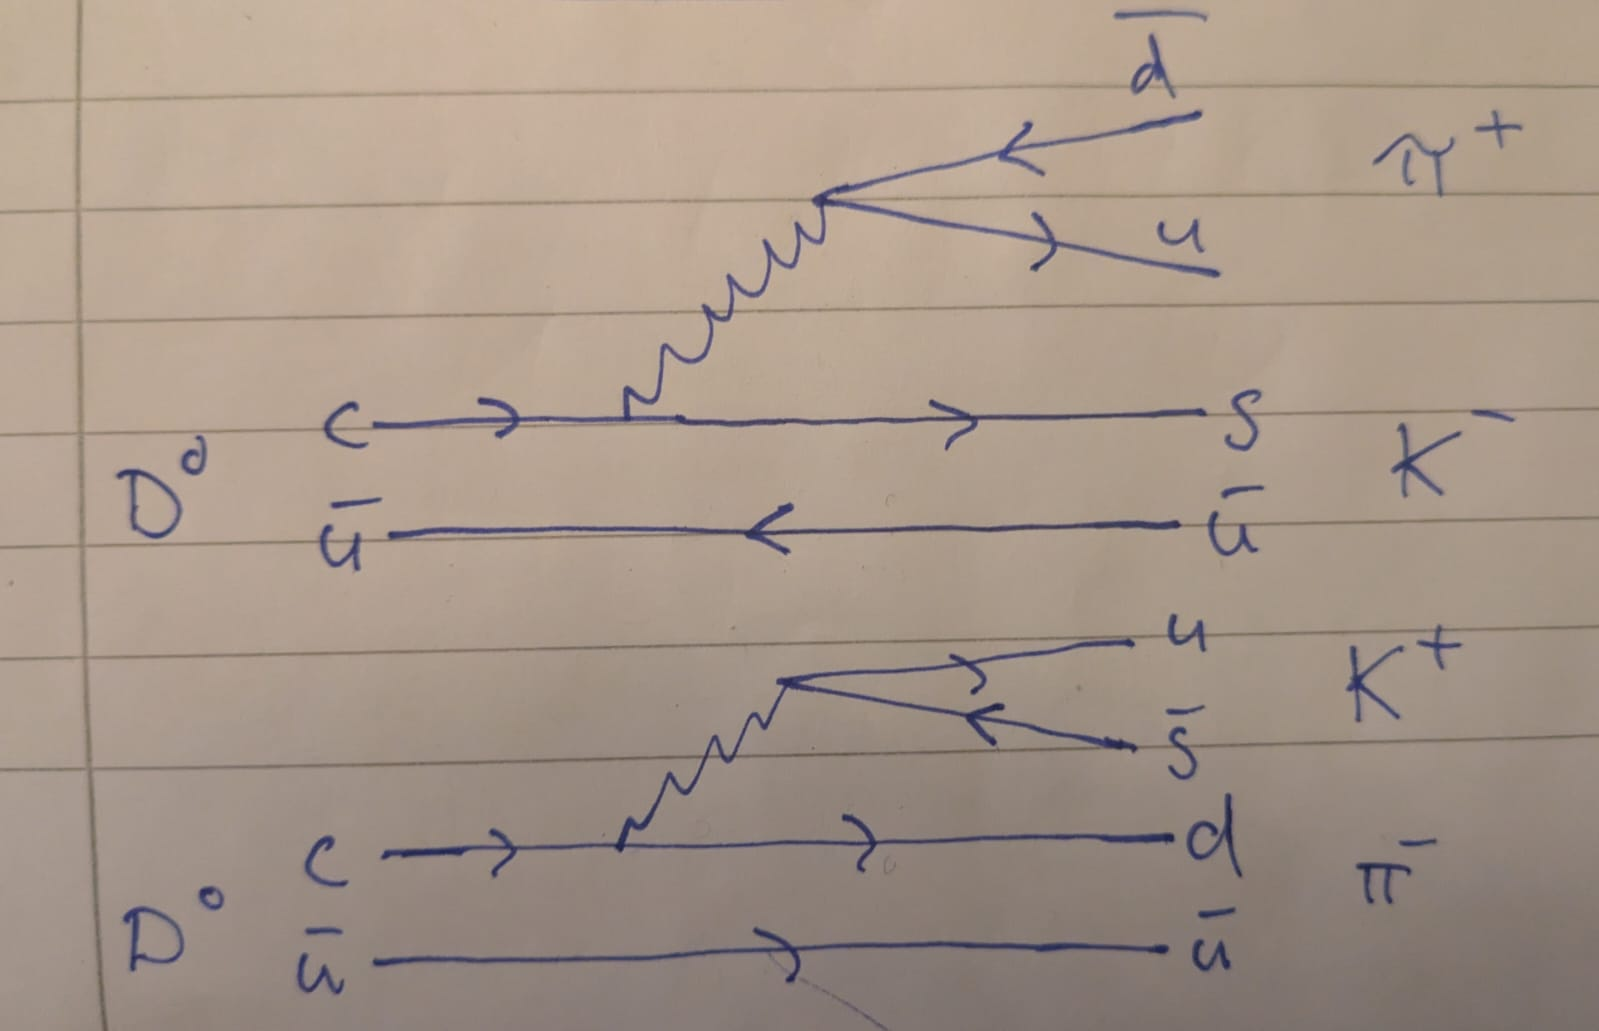
\includegraphics{feynman.jpg}
\caption{feynman diagrams}
\end{figure}

The decay \(D^0 \to K^-\pi^+\) is significantly more likely, because the
transition \(c\to W^+ + s\) does not involve a change in the quark
family. The relevant amplitude of the CKM matrix is therefore on the
diagonal making it the most probable transition. Further more the decay
\(W^+\to \bar d + u\) is also more likely then \(W^+\to \bar s+ u\)
since its transition amplitude also lies on the diagonal.

Mathematically the ration of the decay widths is 
\begin{align*}
    \frac{P(D^0\to K^- + \pi^+)}{P(D^0\to K^+ + \pi^-)}
    &= \frac{|V_{cs}|^2|V_{ud}|^2}{|V_{cd}|^2|V_{us}|^2}\\
    &= \left(\frac{0.97349\cdot 0.97435}{0.22486\cdot 0.22500}\right)^2\\
    &= 351.482
\end{align*}


    \hypertarget{b}{%
\subsection{(b)}\label{b}}

The relative decay widths (source: pdg) are:

\(D^0 \to K^-\pi^+: \ \Gamma_1/\Gamma = (3.947\pm0.030)\cdot10^{-2}\)

\(D^0 \to K^+\pi^-: \ \Gamma_2/\Gamma = (1.363\pm0.025)\cdot 10^{-4}\)

\(\frac{P(D^0\to K^- + \pi^+)}{P(D^0\to K^+ + \pi^-)} = \frac{\Gamma_1}{\Gamma_2} = 289.581\)

The rough estimate for the ration of the decay width, aligns nicely with
the experimental data.


    % Add a bibliography block to the postdoc
    
    
    
\end{document}
